% Options for packages loaded elsewhere
\PassOptionsToPackage{unicode}{hyperref}
\PassOptionsToPackage{hyphens}{url}
%
\documentclass[
]{article}
\usepackage{amsmath,amssymb}
\usepackage{iftex}
\ifPDFTeX
  \usepackage[T1]{fontenc}
  \usepackage[utf8]{inputenc}
  \usepackage{textcomp} % provide euro and other symbols
\else % if luatex or xetex
  \usepackage{unicode-math} % this also loads fontspec
  \defaultfontfeatures{Scale=MatchLowercase}
  \defaultfontfeatures[\rmfamily]{Ligatures=TeX,Scale=1}
\fi
\usepackage{lmodern}
\ifPDFTeX\else
  % xetex/luatex font selection
\fi
% Use upquote if available, for straight quotes in verbatim environments
\IfFileExists{upquote.sty}{\usepackage{upquote}}{}
\IfFileExists{microtype.sty}{% use microtype if available
  \usepackage[]{microtype}
  \UseMicrotypeSet[protrusion]{basicmath} % disable protrusion for tt fonts
}{}
\makeatletter
\@ifundefined{KOMAClassName}{% if non-KOMA class
  \IfFileExists{parskip.sty}{%
    \usepackage{parskip}
  }{% else
    \setlength{\parindent}{0pt}
    \setlength{\parskip}{6pt plus 2pt minus 1pt}}
}{% if KOMA class
  \KOMAoptions{parskip=half}}
\makeatother
\usepackage{xcolor}
\usepackage[margin=1in]{geometry}
\usepackage{longtable,booktabs,array}
\usepackage{calc} % for calculating minipage widths
% Correct order of tables after \paragraph or \subparagraph
\usepackage{etoolbox}
\makeatletter
\patchcmd\longtable{\par}{\if@noskipsec\mbox{}\fi\par}{}{}
\makeatother
% Allow footnotes in longtable head/foot
\IfFileExists{footnotehyper.sty}{\usepackage{footnotehyper}}{\usepackage{footnote}}
\makesavenoteenv{longtable}
\usepackage{graphicx}
\makeatletter
\def\maxwidth{\ifdim\Gin@nat@width>\linewidth\linewidth\else\Gin@nat@width\fi}
\def\maxheight{\ifdim\Gin@nat@height>\textheight\textheight\else\Gin@nat@height\fi}
\makeatother
% Scale images if necessary, so that they will not overflow the page
% margins by default, and it is still possible to overwrite the defaults
% using explicit options in \includegraphics[width, height, ...]{}
\setkeys{Gin}{width=\maxwidth,height=\maxheight,keepaspectratio}
% Set default figure placement to htbp
\makeatletter
\def\fps@figure{htbp}
\makeatother
\setlength{\emergencystretch}{3em} % prevent overfull lines
\providecommand{\tightlist}{%
  \setlength{\itemsep}{0pt}\setlength{\parskip}{0pt}}
\setcounter{secnumdepth}{-\maxdimen} % remove section numbering
\ifLuaTeX
  \usepackage{selnolig}  % disable illegal ligatures
\fi
\usepackage{bookmark}
\IfFileExists{xurl.sty}{\usepackage{xurl}}{} % add URL line breaks if available
\urlstyle{same}
\hypersetup{
  pdftitle={ Causal Effects of Electric Vehicles Around the World},
  hidelinks,
  pdfcreator={LaTeX via pandoc}}

\title{Causal Effects of Electric Vehicles Around the World}
\author{true \and true}
\date{}

\begin{document}
\maketitle

\section{\texorpdfstring{\textbf{Introduction}}{Introduction}}\label{introduction}

In the Global EV Outlook 2024 (EVO2024), published on April 23, 2024,
the IEA projected that by the end of the year, one in every five cars
sold globally would be electric. Worldwide sales of this powertrain
class were expected to peak at 17 million units, reflecting an increase
from 18\% of all car sales in the previous year. While these figures
suggest a world undergoing rapid yet consistent change, they risk
oversimplifying the situation, as the agency also reported that more
than half of all electric vehicles were manufactured in China, a market
that accounted for 60\% of all EV sales during the same period.

The same report also highlighted a critical point: ``The pace at which
electric car sales pick up in emerging and developing economies outside
China will determine their global success.'' While in contrasting
sentiment, the New York Times quoted the director of the Center for
Automotive Research in Bochum, Germany, who observed, ``The Chinese are
winning market share, and the Germans are losing.'' {[}1{]}

By the last quarter of 2024, the European Union had imposed heavy
tariffs on several Chinese automakers, a move aimed at addressing a
growing competitive imbalance, ``starting to hit the safe places that
Western carmakers had,'' with many European factories reportedly
``making fewer cars than they were built to produce.'' Anton Spisak of
the Centre for European Reform {[}2{]} claims that at the core of
China's competitive advantage lies its lower battery production costs, a
significant factor driving its dominance in the EV sector, further
questioning if the EU's course of action was adequate to meet its stated
goal of regaining competitiveness in the automotive industry within a
five-year period.

This geopolitical and economic rivalry raises a pertinent question: if
public perception exalts the triumph of EVs as inevitable, should it not
be possible to explain a substantial portion of EV sales using simple
macroeconomic and demographic indicators? Such a notion suggests that
the EV's rise might be more easily predictable than the complexities of
global competition imply. {[}3{]}

\section{\texorpdfstring{\textbf{Research
Question}}{Research Question}}\label{research-question}

To what extent can macroeconomic and demographic indicators predict the
growth in Electric Vehicle (EV) sales across different countries, and
how do these relationships vary when accounting for individual country
characteristics (Fixed Effects) and unobserved country-specific
heterogeneity (Random Effects)?

\section{\texorpdfstring{\textbf{Methodology}}{Methodology}}\label{methodology}

To address this research question, we initially selected variables based
on the criteria and methodologies outlined in {[}4{]} and {[}5{]}.
Subsequently, we identified and added new variables that we believed
could provide additional insights. Our first step was to evaluate the
relationships among these variables, specifically checking for high
correlations between any of the newly introduced variables and those
from our original selection. The data for this analysis, which included
electric vehicle sales, macroeconomic indicators (e.g., GDP), air
pollution, and renewable energy consumption, was collected from various
sources. {[}6{]} {[}7{]} {[}8{]}

The dataset was mostly complete, with very few missing entries, which
were imputed using linear interpolation of the respective country's time
series. We explored various mathematical transformations, such as
squaring, square roots, logarithms, and first differences, to identify
those that could be useful for our model specification.

We began with a baseline specification that included all academically
validated variables to test different model types using statistical
tests. The model that performed the best on the statistical tests was
then selected, and a final specification that optimized for maximized
explained variance (R²) and minimized robust standard errors was chosen.

The models tested were Pooled OLS, Fixed Effects, Random Effects and
Mixed Effects and the statistical tests were Lagrange Multiplier,
Breusch-Pagan, Robust Hausman and the Breusch--Godfrey Test. When
applicable, robust standard errors were computed using the covariance
matrix appropriate for the statistical properties of each model.

\section{\texorpdfstring{\textbf{Results}}{Results}}\label{results}

The plot shows a clear exponential growth curve with respect to the sale
of electric vehicles, as we would expect, given the analysis provided by
the IEA in EV Outlook 2024. This immediately placed a ceiling on the
expected utility of our modelling, as exponential growth phenomena can
only be approximated by linear models in the short term.

\begin{figure}

{\centering 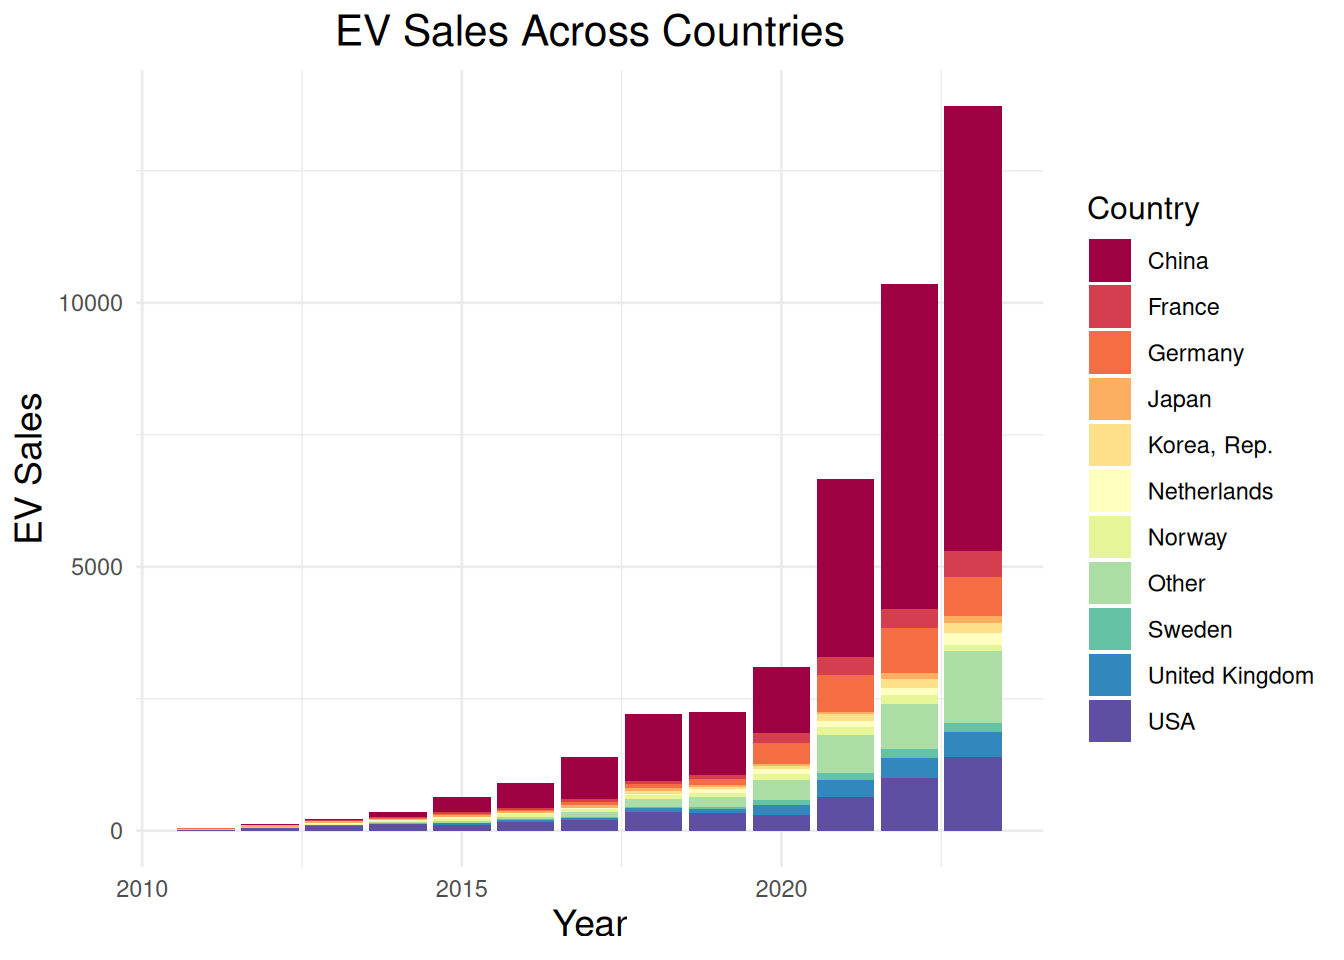
\includegraphics[width=1\linewidth]{poster_markdown_files/figure-latex/unnamed-chunk-2-1} 

}

\caption{Figure 1 - EV Sales across countries}\label{fig:unnamed-chunk-2}
\end{figure}

First, we assessed the presence of panel effects in our data applying
the Lagrange Multiplier test to the Pooled OLS model. Having confirmed
the presence of panel effects, we proceeded to compute the Breush Pagan
and the Breush Godfrey tests for all models. We concluded that there was
heteroskedasticity and residual serial correlation, independent of the
model used. To account for this, we report the robust standard errors
using HC3 - moderately penalizing high leverage observations - and the
Arellano method specifically designed to address the computation of the
covariance matrix under the assumption of heteroskedasticity and serial
correlation.

\begin{longtable}[]{@{}
  >{\raggedright\arraybackslash}p{(\columnwidth - 6\tabcolsep) * \real{0.2703}}
  >{\raggedright\arraybackslash}p{(\columnwidth - 6\tabcolsep) * \real{0.2432}}
  >{\raggedright\arraybackslash}p{(\columnwidth - 6\tabcolsep) * \real{0.2432}}
  >{\raggedright\arraybackslash}p{(\columnwidth - 6\tabcolsep) * \real{0.2432}}@{}}
\caption{Table 1 - Panel Data Analysis}\tabularnewline
\toprule\noalign{}
\begin{minipage}[b]{\linewidth}\raggedright
Test
\end{minipage} & \begin{minipage}[b]{\linewidth}\raggedright
P-value
\end{minipage} & \begin{minipage}[b]{\linewidth}\raggedright
H0
\end{minipage} & \begin{minipage}[b]{\linewidth}\raggedright
Conclusion
\end{minipage} \\
\midrule\noalign{}
\endfirsthead
\toprule\noalign{}
\begin{minipage}[b]{\linewidth}\raggedright
Test
\end{minipage} & \begin{minipage}[b]{\linewidth}\raggedright
P-value
\end{minipage} & \begin{minipage}[b]{\linewidth}\raggedright
H0
\end{minipage} & \begin{minipage}[b]{\linewidth}\raggedright
Conclusion
\end{minipage} \\
\midrule\noalign{}
\endhead
\bottomrule\noalign{}
\endlastfoot
Lagrange Multiplier & 1.726e⁻¹⁰ & No Panel Effects & Has Panel
Effects \\
Breusch Pagan (all models) & 2e⁻¹⁶ & Homoskedasticity &
Heteroskedasticity \\
Breusch Godfrey (all models) & 2e⁻¹⁶ & No Residual Serial Correlation &
Residuals serially correlated \\
Robust Hausman & 0.4675 & Use Random Effects & Use Random Effects \\
\end{longtable}

Below, we report the models results, featuring the estimators'
importance.

\begin{longtable}[]{@{}
  >{\raggedright\arraybackslash}p{(\columnwidth - 10\tabcolsep) * \real{0.1667}}
  >{\raggedright\arraybackslash}p{(\columnwidth - 10\tabcolsep) * \real{0.1667}}
  >{\raggedright\arraybackslash}p{(\columnwidth - 10\tabcolsep) * \real{0.1667}}
  >{\raggedright\arraybackslash}p{(\columnwidth - 10\tabcolsep) * \real{0.1667}}
  >{\raggedright\arraybackslash}p{(\columnwidth - 10\tabcolsep) * \real{0.1667}}
  >{\raggedright\arraybackslash}p{(\columnwidth - 10\tabcolsep) * \real{0.1667}}@{}}
\caption{Table 2 - Estimator importance}\tabularnewline
\toprule\noalign{}
\begin{minipage}[b]{\linewidth}\raggedright
Model
\end{minipage} & \begin{minipage}[b]{\linewidth}\raggedright
gdp
\end{minipage} & \begin{minipage}[b]{\linewidth}\raggedright
pm25exp\_square
\end{minipage} & \begin{minipage}[b]{\linewidth}\raggedright
co2emit
\end{minipage} & \begin{minipage}[b]{\linewidth}\raggedright
co2emit\_diff
\end{minipage} & \begin{minipage}[b]{\linewidth}\raggedright
factor(Country)
\end{minipage} \\
\midrule\noalign{}
\endfirsthead
\toprule\noalign{}
\begin{minipage}[b]{\linewidth}\raggedright
Model
\end{minipage} & \begin{minipage}[b]{\linewidth}\raggedright
gdp
\end{minipage} & \begin{minipage}[b]{\linewidth}\raggedright
pm25exp\_square
\end{minipage} & \begin{minipage}[b]{\linewidth}\raggedright
co2emit
\end{minipage} & \begin{minipage}[b]{\linewidth}\raggedright
co2emit\_diff
\end{minipage} & \begin{minipage}[b]{\linewidth}\raggedright
factor(Country)
\end{minipage} \\
\midrule\noalign{}
\endhead
\bottomrule\noalign{}
\endlastfoot
Pooled OLS & 0.03756 * & 0.03184 * & 2e⁻¹⁶ *** & 2e⁻¹⁶ *** & - \\
FE & 0.008461 ** & 0.009028 ** & 2e⁻¹⁶ *** & 2e⁻¹⁶ *** & - \\
Robust FE & .05482 . & 3.377e⁻⁵ *** & 5.023e⁻⁵ *** & 0.27481 & - \\
RE & 0.03691 * & 0.03123 * & 2e⁻¹⁶ *** & 2e⁻¹⁶ *** & - \\
Robust RE & 0.120033 & 0.020965 * & 0.0007998 *** & 0.361396 & - \\
Mixed FE & 2e⁻¹⁶ *** & 1.653e⁻¹⁴ *** & 2e⁻¹⁶ *** & 2e⁻¹⁶ *** & Yes \\
Robust Mixed FE & 2.388e⁻⁶ *** & 0.2254487 & 5.123e⁻¹⁴ *** & 0.0848060 .
& Yes \\
Mixed RE & 2e⁻¹⁶ *** & 2e⁻¹⁶ *** & 2e⁻¹⁶ *** & 2e⁻¹⁶ *** & Yes \\
Robust Mixed RE & 4.551e⁻⁵ *** & 0.2452769 & 5.227e⁻¹³ *** & 0.1347671 &
Yes \\
\end{longtable}

\begin{longtable}[]{@{}
  >{\raggedright\arraybackslash}p{(\columnwidth - 10\tabcolsep) * \real{0.1667}}
  >{\raggedright\arraybackslash}p{(\columnwidth - 10\tabcolsep) * \real{0.1667}}
  >{\raggedright\arraybackslash}p{(\columnwidth - 10\tabcolsep) * \real{0.1667}}
  >{\raggedright\arraybackslash}p{(\columnwidth - 10\tabcolsep) * \real{0.1667}}
  >{\raggedright\arraybackslash}p{(\columnwidth - 10\tabcolsep) * \real{0.1667}}
  >{\raggedright\arraybackslash}p{(\columnwidth - 10\tabcolsep) * \real{0.1667}}@{}}
\caption{Table 3 - Best Model Specification}\tabularnewline
\toprule\noalign{}
\begin{minipage}[b]{\linewidth}\raggedright
Robust Mixed FE
\end{minipage} & \begin{minipage}[b]{\linewidth}\raggedright
gdp *
\end{minipage} & \begin{minipage}[b]{\linewidth}\raggedright
pm25exp\_square
\end{minipage} & \begin{minipage}[b]{\linewidth}\raggedright
co2emit *
\end{minipage} & \begin{minipage}[b]{\linewidth}\raggedright
co2emit\_diff
\end{minipage} & \begin{minipage}[b]{\linewidth}\raggedright
factor(Country) *
\end{minipage} \\
\midrule\noalign{}
\endfirsthead
\toprule\noalign{}
\begin{minipage}[b]{\linewidth}\raggedright
Robust Mixed FE
\end{minipage} & \begin{minipage}[b]{\linewidth}\raggedright
gdp *
\end{minipage} & \begin{minipage}[b]{\linewidth}\raggedright
pm25exp\_square
\end{minipage} & \begin{minipage}[b]{\linewidth}\raggedright
co2emit *
\end{minipage} & \begin{minipage}[b]{\linewidth}\raggedright
co2emit\_diff
\end{minipage} & \begin{minipage}[b]{\linewidth}\raggedright
factor(Country) *
\end{minipage} \\
\midrule\noalign{}
\endhead
\bottomrule\noalign{}
\endlastfoot
Estimate & 0.46899 & 0.39887 & 0.90779 & -1.9012 & Yes \\
Robust SE & 0.097758 & 0.32847 & 0.11561 & 1.1 & Yes \\
\end{longtable}

The Robust Mixed Fixed Effects (RMFE) model provided a balance between
the performance of the Fixed Effects model while accounting for
heteroskedasticity of the data. It was able to explain 86\% of the
variability (adjusted R² of 0.86) of the outcome variable
(\emph{evsales}), with a very high F-statistic (69.8968, 36, 348),
associated with the low p-value of 2.22e⁻¹⁶, indicating an overall
jointly statistically significant model.

\section{\texorpdfstring{\textbf{Conclusions}}{Conclusions}}\label{conclusions}

Overall, the academically validated variables proved to be a good
baseline for modelling. However, the RMFE model only showed significance
for GDP and CO2 emissions, as well as intrinsic country effects, in the
explanation of electric vehicles sales.

Despite the promising results, because mixed effects models are hard to
compare against fixed effects models directly, under our assumptions, we
fail to conclude definitively on the best model.

Regardless, these results are clear evidence that much of the
variability in the sale of electric vehicles can be explained by making
use of rather simple macroeconomic indicators.

\section{\texorpdfstring{\textbf{Next
Steps}}{Next Steps}}\label{next-steps}

In the future, this work would greatly benefit of testing mixed effects
linear regression models using a more dedicated library, such as
\emph{lme4}, or even other types of non-linear regression models.

\section{\texorpdfstring{\textbf{References}}{References}}\label{references}

\begin{enumerate}
\def\labelenumi{\arabic{enumi}.}
\item
  New York Times Article: Bowles, N. (2024, December 15). Automakers
  face trouble amid electric vehicle shift. The New York Times.
  Retrieved from
  \url{https://www.nytimes.com/2024/12/15/business/automakers-trouble.html}
\item
  Centre for European Reform Article: Centre for European Reform.
  (n.d.). The EU's drive on China: What EV tariffs mean for Europe.
  Retrieved from
  \url{https://www.cer.eu/insights/eus-drive-china-what-ev-tariffs-mean-europe}
\item
  European Commission. (2024). Commission adopts new measures to
  accelerate EV transition and strengthen EU industry. Retrieved from
  \url{https://ec.europa.eu/commission/presscorner/detail/en/ip_24_5589}
\item
  Kovárník, R. \& Staňková, M. Determinants of Electric Car Sales in
  Europe. LOGI -- Scientific Journal on Transport and Logistics, 2021,
  Sciendo, vol.~12 no. 1, pp.~214-225.
  \url{https://doi.org/10.2478/logi-2021-0020}
\item
  Yeh, Jen-Yin \& Wang, Yu-Ting. (2023). A Prediction Model for Electric
  Vehicle Sales Using Machine Learning Approaches. Journal of Global
  Information Management. 31. 1-21. 10.4018/JGIM.327277.
\item
  EV Sales data Sales Info IEA (2024), Global EV Outlook 2024, IEA,
  Paris \url{https://www.iea.org/reports/global-ev-outlook-2023},
  Licence: CC BY 4.0
\item
  World Bank Global Economic Monitor Data World Bank. (2025). Global
  Economic Monitor (GEM). Data retrieved from World Bank DataBank:
  \url{https://databank.worldbank.org/source/global-economic-monitor-(gem)}
\item
  World Bank World Development Indicators Data World Bank. (2025). World
  Development Indicators (WDI). Data retrieved from World Bank DataBank:
  \href{https://databank.worldbank.org/source/global-economic-monitor-(gem)}{https://databank.worldbank.org/source/}\href{https://databank.worldbank.org/source/world-development-indicators}{world-development-indicators}
\end{enumerate}

\end{document}
